\documentclass{VUMIFPSkursinis}
\usepackage{algorithmicx}
\usepackage{algorithm}
\usepackage{algpseudocode}
\usepackage{amsfonts}
\usepackage{amsmath}
\usepackage{bm}
\usepackage{caption}
\usepackage{color}
\usepackage{float}
\usepackage{graphicx}
\usepackage{listings}
\usepackage{subfig}
\usepackage{wrapfig}

\usepackage{enumitem}
%PAKEISTA, tarpai tarp sąrašo elementų
\setitemize{noitemsep,topsep=0pt,parsep=0pt,partopsep=0pt}
\setenumerate{noitemsep,topsep=0pt,parsep=0pt,partopsep=0pt}

% Titulinio aprašas
\university{Vilniaus universitetas}
\faculty{Matematikos ir informatikos fakultetas}
\department{Programų sistemų katedra}
\papertype{Programų sistemų inžinerijos I laboratorinis darbas Nr. 1}
\title{Kavinės staliuko rezervavimo aplikacija}
\titleineng{Cafe table rezervation app}
\status{2 kurso 5 grupės studentai}
\author{Paulius Grigaliūnas}
\secondauthor{Karolis Staskevičius}
\thirdauthor{Modestas Dulevičius}
\fourthauthor{Albert Jurkoit}
\fifthauthor{Šarūnas Kazimieras Buteikis}
     

% \secondauthor{Vardonis Pavardonis}   % Pridėti antrą autorių
\supervisor{dr. Vytautas Valaitis}
\date{Vilnius – \the\year}

% Nustatymai
% \setmainfont{Palemonas}   % Pakeisti teksto šriftą į Palemonas (turi būti įdiegtas sistemoje)
\bibliography{bibliografija}

\begin{document}
	
% PAKEISTA	
\maketitle
\cleardoublepage\pagenumbering{arabic}
\setcounter{page}{2}


%ANOTACIJA

\sectionnonum{ANOTACIJA}
{\bfseries Darbo tikslas:} sukurti išmanų, patogų kavinių staliukų rezervavimo programėlės modelį, kuris funkcionuotų Windows ir Android sistemose. Taip pat siekiama, kad galutinė programėlė užtikritnų sklandų, spartų komunikabilumą tarp klientų ir kavinės darbuotojų, suteikiant galimybę kavinių savininkams pateikti išsamų kavinės planą, o klientams išsirinkti norimą staliuką kavinėje patiems. 
\newline
\newline
\newline

%DARBO ATLIKO

{\bfseries Darbą atliko:}
\newline
\newline
\newline
Paulius Grigaliūnas
\newline
paulius.grigaliunas.pg@gmail.com
\newline
\newline
\newline
Karolis Staskevičius
\newline
karolio paštas
\newline
\newline
\newline
Modestas Dulevičius
\newline
modes paštas
\newline
\newline
\newline
Albert Jurkoit
\newline
albert.jurkoit@mif.stud.vu.lt
\newline
\newline
\newline
Šarūnas Kazimieras Buteikis
\newline
sarunas.kazimieras.buteikis@gmail.com

%TURINYS

\tableofcontents

%ĮVADAS

\sectionnonum{Įvadas}
\noindent
{\bfseries "Book a Table" kavinės rezervavimo aplikacija}
\newline
\newline
{\bfseries Dalykinė sritis}
\newline
Kavinės ir jų rezervacija
\newline
\newline
{\bfseries Probleminė sritis}
\newline
 Lietuvoje staliuko rezervavimo galimybės yra mažai praplėstos
\newline
\newline
{\bfseries Naudotojai}
\newline
Žmonės, norintys skaniai pavalgyt, bei iš anksto pasirūpint vietą restorane.
\newline
Kavynių savininkai, suteikiantys žmonėms galimybę rezervuoti staliuką jų restorane.
\newline
\newline
{\bfseries Darbo pagrindas}
\newline
Dokumentas parengtas kaip programų sistemų inžinerios dalyko laboratorinis darbas Nr. 1, kuriame pateikiamas suprojektuotos sistemos aprašymas.
\newline
\newline

\section{Programų sistemos architektūra}
%LOGINIS PJUVIS
\subsection{Loginis pjūvis}
%KLASIU DIAGRAMA
\subsubsection{Klasių diagrama}



Žemiau pateikta


\begin{figure}[H]
    \centering
    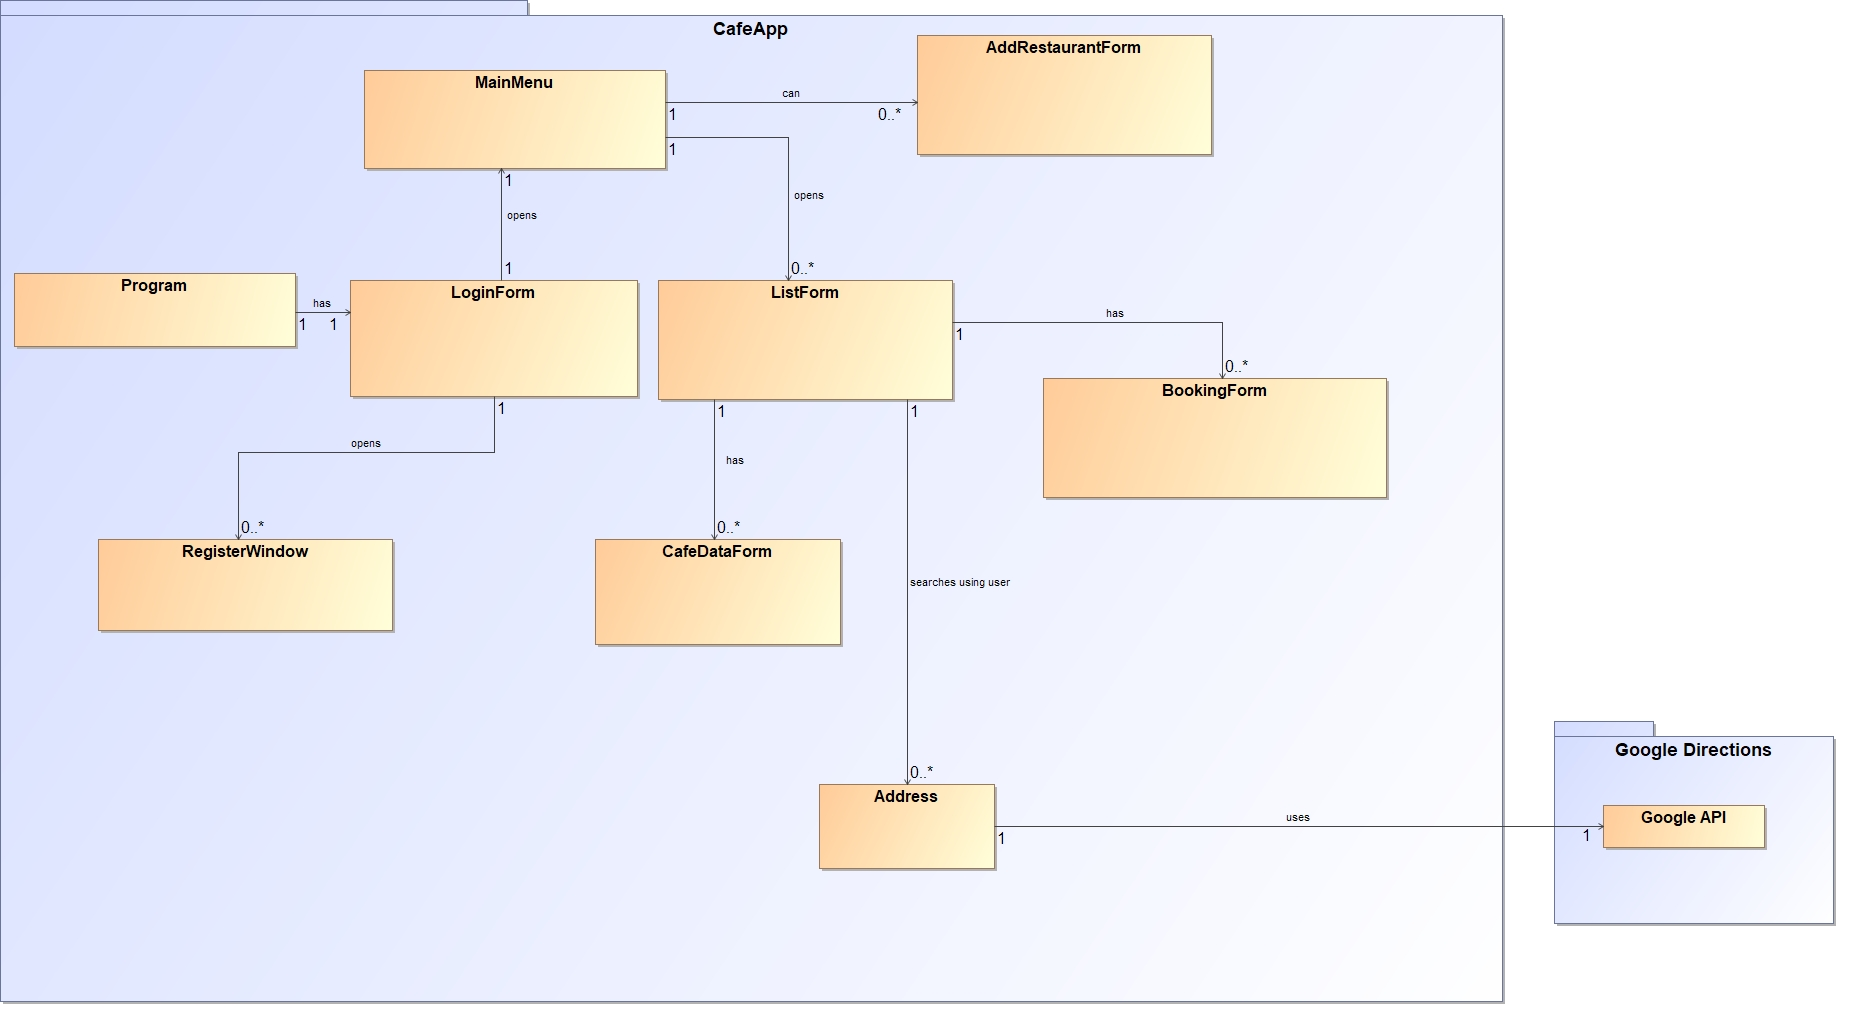
\includegraphics[width=\textwidth,height=\textheight,keepaspectratio]{img/Model} 
    \caption{Klasių diagrama}
    \label{img:Model}
\end{figure}

%OBJEKTU DIAGRAMA
\subsubsection{Objektų diagrama}

\subsection{Dinaminis programų sistemos modelis (angl. Process view)}
\subsubsection{Veiklos diagramos}
\begin{figure}[H]
    \centering
    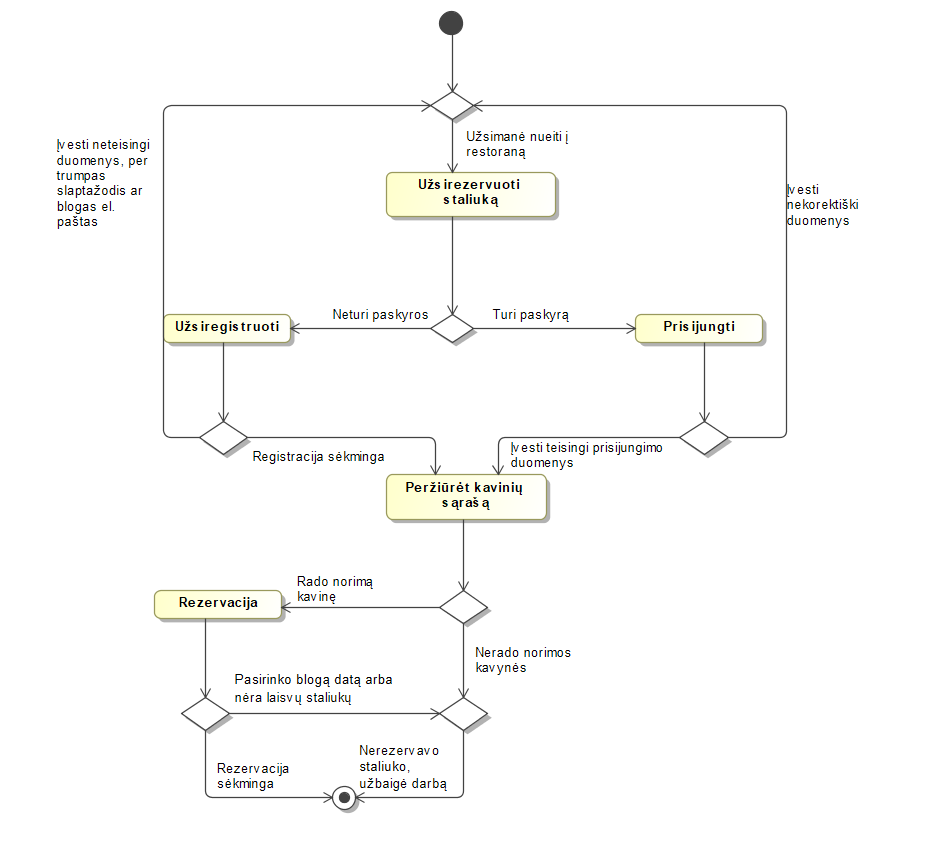
\includegraphics[width=\textwidth,height=\textheight,keepaspectratio]{img/rezerv} 
    \caption{Kavinės rezervacijos veiklos diagrama}
    \label{img:rezerv}
\end{figure}
% Vietoj x įrašyt real sk.
x pav.   diagramoje nagrinėjami procesai, vykstantys tuo metu, kai vartotojas nori rezervuoti staliuką kavinėje. Rezervacija yra pasiekiama tik po prisijungimo arba užsiregistravimo sistemoje. Vartotojas pamato prisijungimo ir registracijos opcijas tik paleidęs aplikaciją. Būsimas sistemos narys privalo užpildyti registracijos formą, parinkti saugų slaptažodį, bei nurodyt egzistuojantį el. paštą. Užpildžius formą neteisingai, reikia pakeisti netinkamus laukus. Sėkmingai prisijungus prie sistemos, vartotojas gali peržiūrėti aplikacijoje užregistruotų kavinių sąrašą. Jeigu vartotojas randa jam patinkančią kavinę, jis užpildo rezervavimo formą. Jeigu formoje visi laukai yra nurodyti teisingai ir restorane yra laisvų staliukų - rezervacija yra sėkminga. Darbas yra baigiamas tuo metu, kai vartotojas sėkmingai užsirezervavo staliuką, arba nusprendė nutraukt rezervaciją.


\begin{figure}[H]
    \centering
    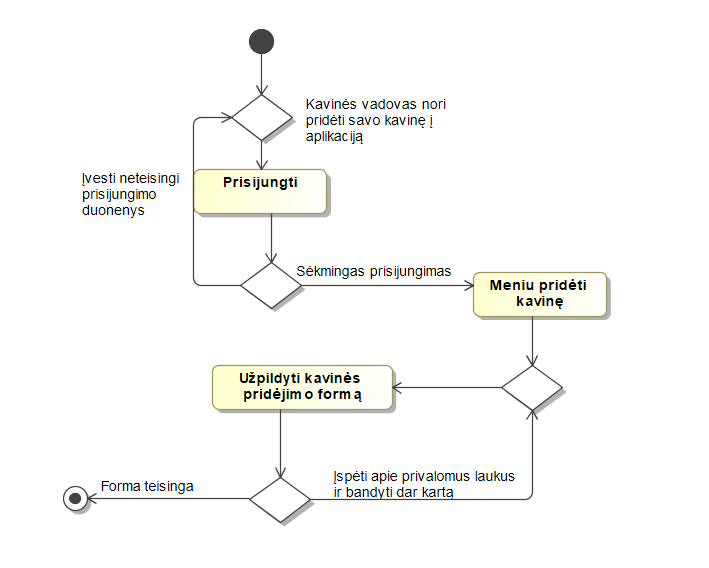
\includegraphics[width=\textwidth,height=\textheight,keepaspectratio]{img/addcafe} 
    \caption{Kavinės pridėjimo prie sistemos veiklos diagrama}
    \label{img:addcafe}
\end{figure}
% Vietoj x įrašyt real sk.
x pav.   diagramoje nagrinėjami procesai, vykstantys vartotojui į sistemą pridedant kavinę. Norint pridėt kavinę į kavinių sąrašą, vartotojui būtina prisijungti (o neturint prisijungimo - prisiregistruoti) prie sistemos. Prisijungus meniu spaudžiama ant "Add cafe" mygtuko ir užpildoma kavinės pridėjimo formą. Jeigu visi laukai pažymėti "*" (būtini) yra užpildyti - kavinė yra pridedama prie sąrašo. 

\begin{figure}[H]
    \centering
    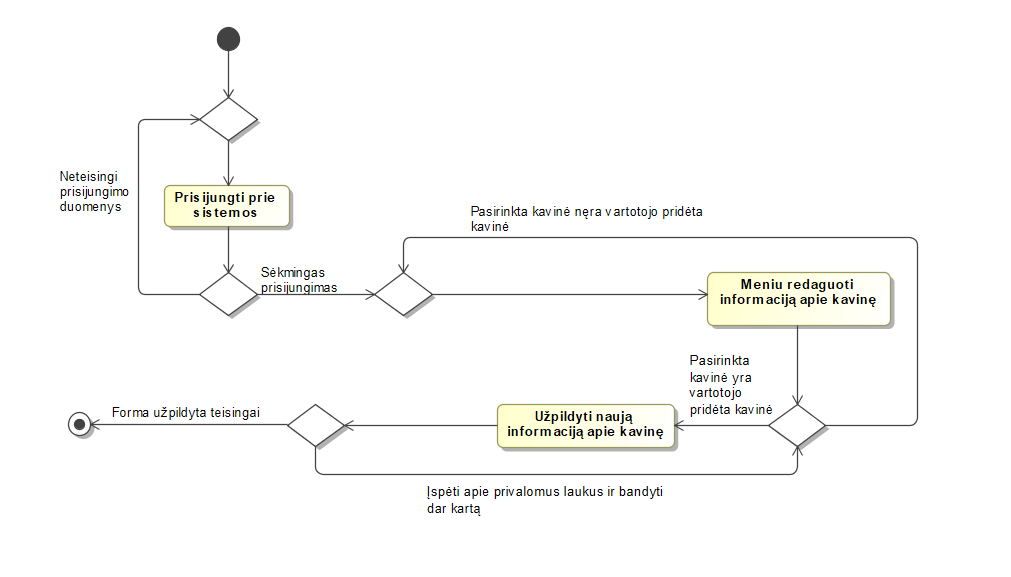
\includegraphics[width=\textwidth,height=\textheight,keepaspectratio]{img/editcafe} 
    \caption{Informacijos apie kavinę redagavimo veiklos diagrama}
    \label{img:editcafe}
\end{figure}
% Vietoj x įrašyt real sk.
x pav.   diagramoje nagrinėjami procesai, vykstantys vartotojui norint pakeist arba atnaujint informaciją apie kavinę. Norint redaguot kavinės informaciją, vartotojui būtina prisijungti prie sistemos. Vartotojas atidaro visų kavinių sąrašą ir pasirinkus savo kavinė ir paspaudus mygtuką "Show info" jis gauna informacija apie jo kavinę bei apačioje formą, kuria teisingai užpildžius ir paspaudus mygtuką "Change" galima atnaujint/pakeist egzistuojančią informaciją apie kavinę.

% DETI CIA SAVO DUOMENIS



\subsection{Programų sistemos išskirstymas tinkle(angl. Deployment view)}
\subsubsection{Komponentų ryšių su artefaktais diagrama}

Žemiau pateiktoje komponentų ryšių su artefaktais diagramoje yra išskirti pagrindiniai sistemos artefaktai. Artefaktus (angl. “artifact”) ir komponentus (angl. “component”) tarpusavyje sieja manifestacijos (angl. “Manifest”) ryšys. Tai reiškia, kad artefakto sudaromoji dalis yra konkretus komponentas.


%Komponentų ryšių su artefaktais diagrama
\begin{figure}[H]
    \centering
    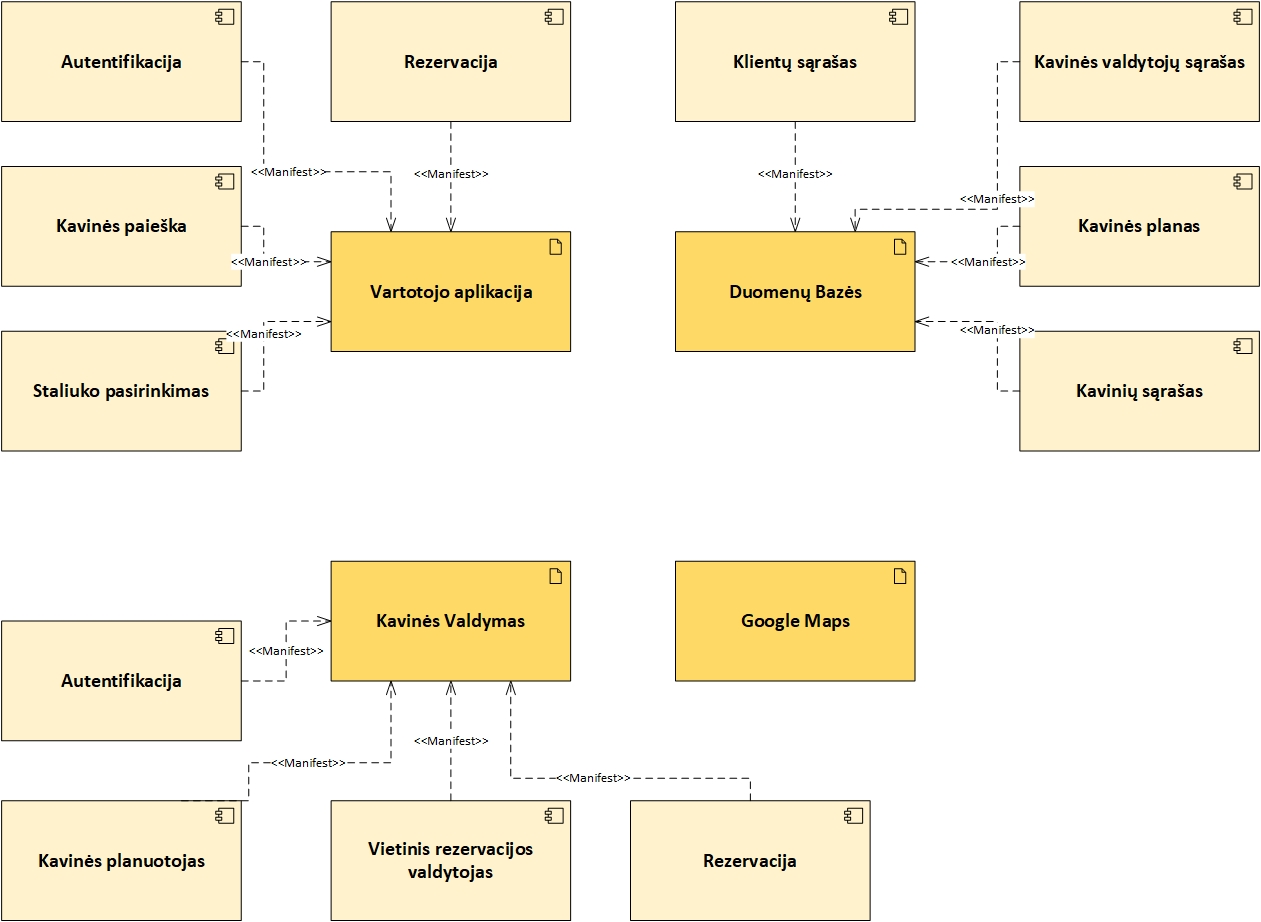
\includegraphics[width=\textwidth,height=\textheight,keepaspectratio]{img/Deployment_diagram1} 
    \caption{Komponentų ryšių su artefaktais diagrama}
    \label{img:Model}
\end{figure}

Sistema susideda iš trijų pagrindinių dalių - Registracijos / Prisijungimo sitemos, kavinės pridėjimo sistemos bei kavinės staliuko rezervacijos sistemos. Visos kavinės programėlės pagrindas susideda iš trijų karkasų: Registracijos / Prisijungimo sistema, Kavinės pridėjimo sistema ir  Kavinės staliuko rezervacijos sistema.


Registracijos / Prisijungimo sistema užtikina kiekvieno vartotojo (kliento ar kavinės vadovo) sklandų prisijungimą prie sistemos. Componentas Kantoleris užtikina, kad kiekvieno prisiregistravusiojo duomenys būtų autentiški. Taip pat registracijoje yra galimybė užsiregistruoti kaip klientas arba kavinės savininkas.

Kavinės pridėjimo Sistema - aktuali programėlės vartotojams prisiregistravusiems kaip kavinės savininkas. Ši Sistema užtikina turimų duomenų apie užregistruotas kavinies saugumą. 

Klientams yra prienama Kavinės staliuko rezervacijos sistema. Šis karkasas yra nesudėtingas, gali būti laisvai naudojamas, skirtas užtikinti klientų konfortą ir garantuotų rezervacijos stabilumą. Jį sudaro trys pagrindiniai komponentai - kontroleris, Informacija apie kavinę, staliuko rezervacija. Staliuko rezervacija yra esminis komponentas šioje sistemoje. Jis leidžia klientui užsirezervuoti norimą staliuką, pasirinktu laiku. Kontroleris užtikina, kad nebūtų suteikiama užsisakyti staliuko tuo pačiu metu kelis kartus skirtingiems klientams. Detalią informaciją apie kavinių sąrašą, jų buvimo vietą, contaktus bei detalesnę informaciją pateikia komponentas pavadinimu - "Informacija apie kavinę".
 
 Naudojantis “Symfony” teikiamomis bibliotekomis ir interfeisais, buvo sukurta pati knygų dalinimosi sistema. Ją sudaro keturi pagrindiniai komponentai - kontroleriai, vartotojo autentifikavimo modulis, prašymų modulis bei knygų peržiūros ir modifikavimo modulis. Kad galėtumėme išsaugoti prašymus dėl knygų atidavimoarbapaieškos,pasirinktaMySQLduomenųbazė.
 
 
 
Artefaktas - Failas arba failų rinkinys,atsakingas už kurią nors sistemos veikimo dalį. 
Manifestacijos(angl. “Manifest”)ryšys- Nurodo,kad artefaktas negali egzistuoti be komponento, su kuriuo jis yra susietas šiuo ryšiu.


\subsubsection{Mazgų diagrama}

%Mazgų diagrama
\begin{figure}[H]
    \centering
    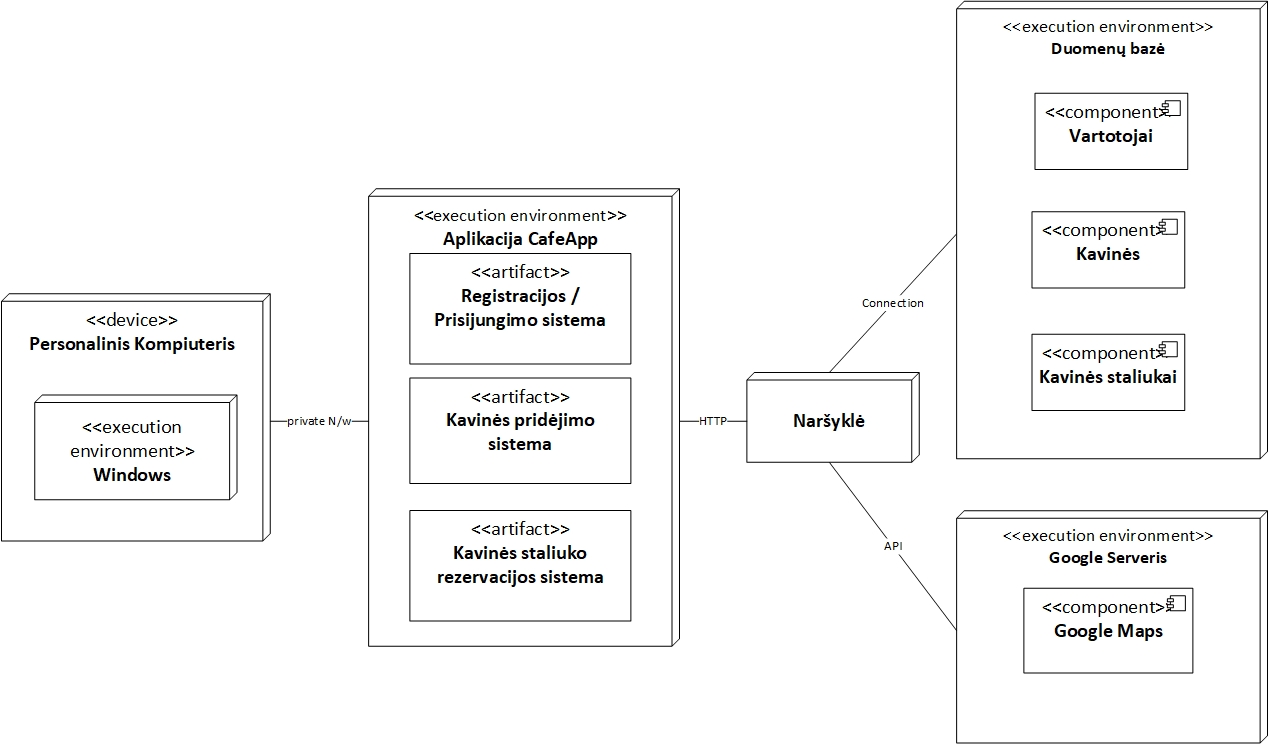
\includegraphics[width=\textwidth,height=\textheight,keepaspectratio]{img/Deployment_diagram2} 
    \caption{Mazgų diagrama}
    \label{img:Model}
\end{figure}



\section{Medžiagos darbo tema dėstymo skyriai}
Medžiagos darbo tema dėstymo skyriuose pateikiamos nagrinėjamos temos detalės:
pradinė medžiaga, jos analizės ir apdorojimo metodai, sprendimų įgyvendinimas,
gautų rezultatų apibendrinimas. Šios dalies turinys labai priklauso nuo darbo
temos. Skyriai gali turėti poskyrius ir smulkesnes sudėtines dalis, kaip
punktus ir papunkčius.

Medžiaga turi būti dėstoma aiškiai, pateikiant argumentus. Tekstas dėstomas
trečiuoju asmeniu, t.y. rašoma ne „aš manau“, bet „autorius mano“, „autoriaus
nuomone“. Reikėtų vengti informacijos nesuteikiančių frazių, pvz., „...kaip jau
buvo minėta...“, „...kaip visiems žinoma...“ ir pan., vengti grožinės literatūros
ar publicistinio stiliaus, gausių metaforų ar panašių meninės išraiškos
priemonių.

\subsection{Poskyris}
Citavimo pavyzdžiai: cituojamas vienas šaltinis \cite{PvzStraipsnLt}; cituojami
keli šaltiniai \cite{PvzStraipsnEn, PvzKonfLt, PvzKonfEn, PvzKnygLt, PvzKnygEn,
PvzElPubLt, PvzElPubEn, PvzMagistrLt, PvzPhdEn}.

\begin{enumerate}
	\item Pirmas elementas
	\item Antras elementas
\end{enumerate}

Lorem ipsum dolor sit amet, consectetur adipiscing elit. Curabitur at mauris sit amet nisi vestibulum tincidunt non vel mi. Pellentesque lacinia, sapien id sollicitudin egestas, diam erat dapibus justo, a cursus arcu nunc feugiat sapien. Mauris elit lorem, egestas at nisl at, consequat tempus nisi. Aliquam congue consectetur lorem ut venenatis. Suspendisse scelerisque eros ac sapien pulvinar, id fermentum sem bibendum. Phasellus rhoncus nec tellus quis gravida. Fusce at nibh porta, sodales ipsum quis, facilisis velit. Phasellus semper laoreet magna, eget eleifend massa. Donec sollicitudin risus risus, sodales dignissim ex bibendum et. Aliquam neque lectus, posuere vitae suscipit et, hendrerit eu mauris. Integer cursus neque ex, sed molestie ex suscipit et. Phasellus eget quam id arcu tincidunt fringilla eget eu tortor. In hac habitasse platea dictumst.


\subsubsection{Skirsnis}
\subsubsubsection{Straipsnis}
\subsubsection{Skirsnis}
\section{Skyrius}
\subsection{Poskyris}
\subsection{Poskyris}

\sectionnonum{Rezultatai ir išvados}
Šiame laboratoriniame darbe pasitelkiant skirtingus sistemos pjūvius aprašyta kavinių rezervavimo sistemos architektūra. Loginis pjūvis leido išskirti pagrindines esybes bei ryšius tarpjų. Kūrimo pjūvyje atlikta sistemos dekompozicija pradedant nuo bendro komponento toliaujį detalizuojant. Užduočių pjūvyje išsiaiškinti pagrindiniai agentų tikslai naudojantis sistema.Fiziniame pjūvyje apibrėžtas sistemos išdėstymas tinkle.  Galiausiai procesų pjūvyje išskirtiprocesai, jų komunikacija. Šis skirtingų požiūrių rinkinys leido iš ankstoaptikti sistemoje galimas klaidas bei sukurti tinkamą sistemos architektūrą.

%% PAKEISTAS PAVADINIMAS Į 'Šaltiniai'
\printbibliography[heading=bibintoc, title=Šaltiniai]  % Šaltinių sąraše nurodoma panaudota
% literatūra, kitokie šaltiniai. Abėcėlės tvarka išdėstomi darbe panaudotų
% (cituotų, perfrazuotų ar bent paminėtų) mokslo leidinių, kitokių publikacijų
% bibliografiniai aprašai.  Šaltinių sąrašas spausdinamas iš naujo puslapio.
% Aprašai pateikiami netransliteruoti. Šaltinių sąraše negali būti tokių
% šaltinių, kurie nebuvo paminėti tekste.

% \sectionnonum{Sąvokų apibrėžimai}
\sectionnonum{Santrumpos}
Sąvokų apibrėžimai ir santrumpų sąrašas sudaromas tada, kai darbo tekste
vartojami specialūs paaiškinimo reikalaujantys terminai ir rečiau sutinkamos
santrumpos.

\appendix  % Priedai
% Prieduose gali būti pateikiama pagalbinė, ypač darbo autoriaus savarankiškai
% parengta, medžiaga. Savarankiški priedai gali būti pateikiami ir
% kompaktiniame diske. Priedai taip pat numeruojami ir vadinami. Darbo tekstas
% su priedais susiejamas nuorodomis.

\section{Neuroninio tinklo struktūra}
\begin{figure}[H]
    \centering
    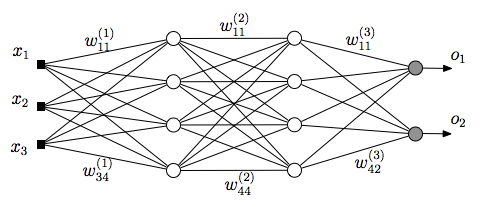
\includegraphics[scale=0.5]{img/MLP}
    \caption{Paveikslėlio pavyzdys}
    \label{img:mlp}
\end{figure}


\section{Eksperimentinio palyginimo rezultatai}
% tablesgenerator.com - converts calculators (e.g. excel) tables to LaTeX
\begin{table}[H]\footnotesize
  \centering
  \caption{Lentelės pavyzdys}
  {\begin{tabular}{|l|c|c|} \hline
    Algoritmas & $\bar{x}$ & $\sigma^{2}$ \\
    \hline
    Algoritmas A  & 1.6335    & 0.5584       \\
    Algoritmas B  & 1.7395    & 0.5647       \\
    \hline
  \end{tabular}}
  \label{tab:table example}
\end{table}

\end{document}
